\documentclass[a4paper, 10pt]{article}

\usepackage[a4paper, total={6in, 8.5in}]{geometry}

\usepackage[utf8]{inputenc}
\usepackage{graphicx} 
\usepackage{verbatim} 
\usepackage{float}
\usepackage{xfrac}
\usepackage{mathpazo}
\usepackage{amsmath}
\usepackage{bm}

\usepackage{multicol}
\usepackage{sectsty,textcase}

\usepackage{wrapfig,lipsum,booktabs}
\bibliographystyle{plain}
% \renewcommand{\thesubsection}{\alph{subsection})}
\renewcommand{\thesection}{\arabic{section}}

%\setlength\parindent{0pt}	

\title{FYS-STK3155/4155 Applied Data Analysis and Machine Learning - Project 1: Regression analysis and resampling methods }

\author{Bernhard Nornes Lotsberg, Anh-Nguyet Lise Nguyen}
\date{September 2019}
\begin{document}
\maketitle


\begin{abstract} %\noindent
    this project blah blah blah\\
    Lorem ipsum dolor sit amet, consectetur adipiscing elit. Fusce et semper nibh, in vehicula sapien. In ultricies mollis enim, non venenatis odio ullamcorper id. Nunc consequat vulputate tempus.
\end{abstract}

\begin{multicols}{2}
\section{Introduction}



Lorem ipsum dolor sit amet, consectetur adipiscing elit. Fusce et semper nibh, in vehicula sapien. In ultricies mollis enim, non venenatis     odio ullamcorper id. Nunc consequat vulputate tempus. Proin tempus sodales diam. Vestibulum pulvinar, dui et cursus dignissim, est elit placerat metus, sit amet volutpat lacus nisi sed neque. Fusce ullamcorper, sapien sit amet mollis semper, tellus risus luctus mauris, scelerisque blandit justo metus nec dui. Etiam consectetur ex ut elit condimentum, vel dictum mi volutpat. Cras lectus ante, venenatis sit amet nunc sed, auctor convallis lacus. Praesent ut nisi arcu. Morbi blandit ligula non dignissim dapibus. Fusce arcu tellus, sodales at sollicitudin sit amet, rhoncus luctus ex. Integer eget sem quis metus vestibulum accumsan quis vel magna. Integer venenatis pellentesque ex. Aliquam nec semper sapien. Donec tempor vehicula leo, at dictum dui venenatis non.


\section{Theory}
\subsection{Linear regression methods}
If data is assumed to be on the form
\[
Y = f(X)+ \varepsilon 
\]
where $\varepsilon \sim N(0,\ \sigma ^2)$, then a model for the data can be on the form

\[
\hat{Y} = \bm{X}^T\hat{\beta}.
\]
It is possible to approach this problem using various different regression methods. One of the simplest methods is the Ordinary Least Squares (OLS) regression, which minimizes the expression
\begin{equation}
    \hat{\beta}^\text{OLS} = \text{argmin}_{ {\beta} } \left[ \frac{1}{n} \sum_i^n (y_i - X_{i*}^T \beta)^2 \right],
    \label{eq:argminbeta_OLS}
\end{equation}
giving an analytical expression for the optimal regression parameters
\begin{equation}
    \hat{\beta}^{\text{OLS}} = (\bm{X}^T\bm{X})^{-1} \bm{X}^T \bm{y}.
    \label{eq:beta_OLS}
\end{equation}
Ridge regression
\begin{equation}
    \hat{\beta}^\text{ridge} = \text{argmin}_\beta \left[ \frac{1}{n}\sum_i^n(y_i-X_{i*}^T\beta)^2 + \lambda ||\beta||_2^2  \right]
    \label{eq:argminbeta_ridge}
\end{equation}
with the analytical optimal regression parameters
\begin{equation}
    \hat{\beta}^\text{ridge} = (\bm{X}^T\bm{X} +\lambda \bm{I})^{-1} \bm{X}^T \bm{y}.
    \label{eq:beta_ridge}
\end{equation}
The Least Absolute Shrinkage and Selection Operator (LASSO) regression minimizes
\begin{equation}
    \hat{\beta}^\text{lasso} =  \text{argmin}_\beta \left[  \frac{1}{n}\sum_i^n(y_i-X_{i*}^T\beta)^2 + \lambda ||\beta||_1  \right].
    \label{eq:argminbeta_lasso}
\end{equation}

\subsection{Resampling}
When working with limited amounts of data, 


k-fold cross-validation
\section{Method}
Donec elementum tempor eros, in gravida massa scelerisque ut. Vestibulum facilisis metus at ornare commodo. Donec lacus eros, dapibus id nunc id, suscipit ullamcorper justo. In vel felis mauris. Integer ultricies dolor quis vehicula ultricies. Pellentesque mattis elit quis tempus ullamcorper. Donec a nulla orci. Quisque pretium mauris vitae ipsum aliquet, quis malesuada est viverra. Maecenas quis consequat diam, vitae hendrerit tellus. Donec vulputate erat massa, id sollicitudin tellus cursus ut. Aliquam dui justo, interdum ut efficitur suscipit, ullamcorper eget nisi. Ut gravida, tortor at ornare suscipit, lacus tellus malesuada metus, vel lacinia justo lorem in nisl. Donec et sem eget lacus egestas auctor. Integer egestas, lorem eget volutpat malesuada, est nunc efficitur mi, ac pulvinar elit libero quis risus. Aenean convallis aliquam eros, interdum molestie sapien pretium sit amet. Aliquam at aliquam diam.
\begin{equation}
    MSE(\hat{y},\hat{\tilde{y}}) = \frac{1}{n}
    \sum_{i=0}^{n-1}(y_i-\tilde{y}_i)^2, 
    \label{eq:MSE}
\end{equation}
\begin{equation}
    R^2(\hat{y}, \tilde{\hat{y}}) = 1 - \frac{\sum_{i=0}^{n - 1} (y_i - \tilde{y}_i)^2}{\sum_{i=0}^{n - 1} (y_i - \bar{y})^2},
    \label{eq:R2}
\end{equation}


\section{Results}
Donec elementum tempor eros, in gravida massa scelerisque ut. Vestibulum facilisis metus at ornare commodo. Donec lacus eros, dapibus id nunc id, suscipit ullamcorper justo. In vel felis mauris. Integer ultricies dolor quis vehicula ultricies. Pellentesque mattis elit quis tempus ullamcorper. Donec a nulla orci. Quisque pretium mauris vitae ipsum aliquet, quis malesuada est viverra. Maecenas quis consequat diam, vitae hendrerit tellus. Donec vulputate erat massa, id sollicitudin tellus cursus ut. Aliquam dui justo, interdum ut efficitur suscipit, ullamcorper eget nisi. Ut gravida, tortor at ornare suscipit, lacus tellus malesuada metus, vel lacinia justo lorem in nisl. Donec et sem eget lacus egestas auctor. Integer egestas, lorem eget volutpat malesuada, est nunc efficitur mi, ac pulvinar elit libero quis risus. Aenean convallis aliquam eros, interdum molestie sapien pretium sit amet. Aliquam at aliquam diam.


\end{multicols}

\begin{figure}[t!]
    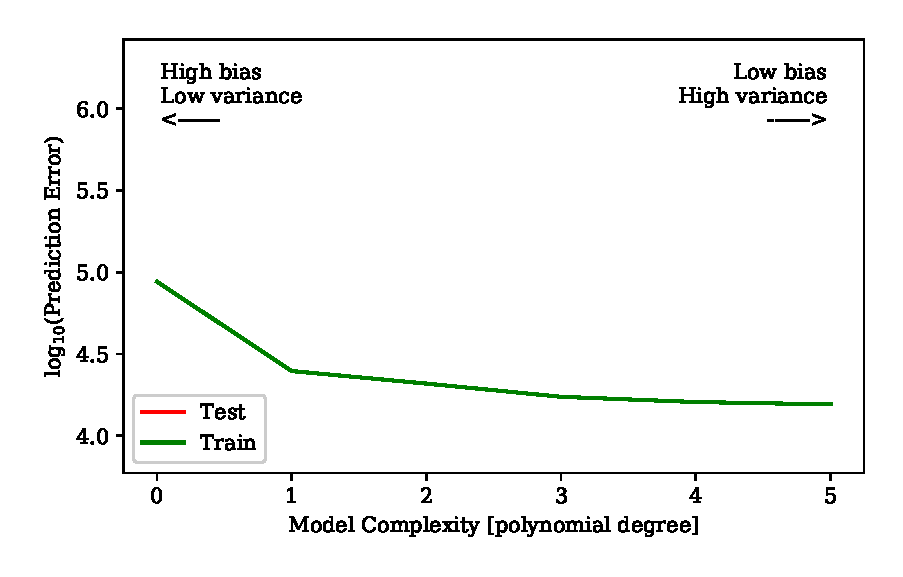
\includegraphics[scale=1]{figs/biasvariancetradeoff.eps}
    \caption{Prediction error of training and test set plotted as a function of model complexity (polynomial degree) for the ordinary least squares regression.}
    \label{fig:my_label}
\end{figure}
    
\begin{figure}[h]
    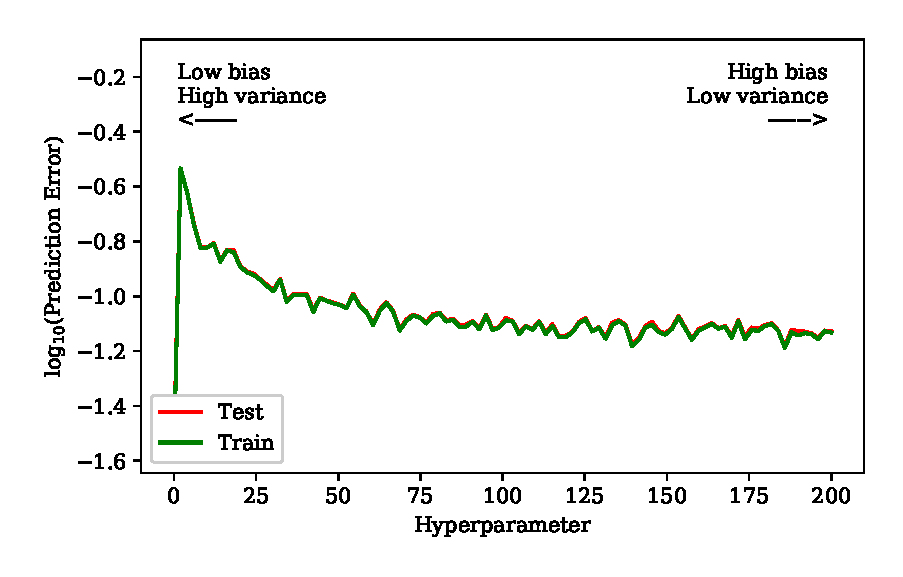
\includegraphics{figs/biasvariancetradeoff_Ridge.eps}
    \caption{Prediction error of training and test set plotted as a function of the hyperparameter $\lambda$ for Ridge regression.}
\end{figure}    

\begin{figure}[h]
    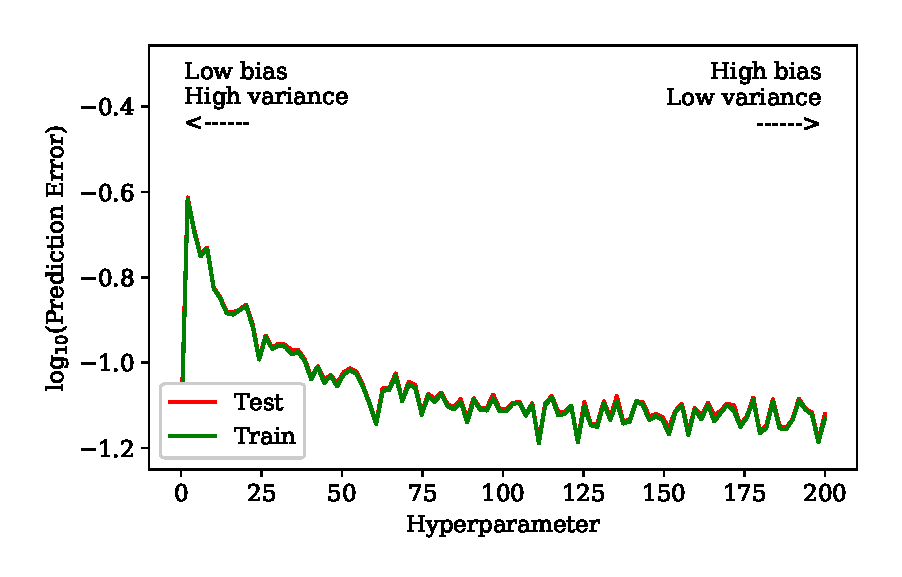
\includegraphics{figs/biasvariancetradeoff_LASSO.eps}
    \caption{Prediction error of training and test set plotted as a function of the hyperparameter $\lambda$ for Lasso regression.}
\end{figure} 

\begin{multicols}{2}

Donec elementum tempor eros, in gravida massa scelerisque ut. Vestibulum facilisis metus at ornare commodo. Donec lacus eros, dapibus id nunc id, suscipit ullamcorper justo. In vel felis mauris. Integer ultricies dolor quis vehicula ultricies. Pellentesque mattis elit quis tempus ullamcorper. Donec a nulla orci. Quisque pretium mauris vitae ipsum aliquet, quis malesuada est viverra. Maecenas quis consequat diam, vitae hendrerit tellus. Donec vulputate erat massa, id sollicitudin tellus cursus ut. Aliquam dui justo, interdum ut efficitur suscipit, ullamcorper eget nisi. Ut gravida, tortor at ornare suscipit, lacus tellus malesuada metus, vel lacinia justo lorem in nisl. Donec et sem eget lacus egestas auctor. Integer egestas, lorem eget volutpat malesuada, est nunc efficitur mi, ac pulvinar elit libero quis risus. Aenean convallis aliquam eros, interdum molestie sapien pretium sit amet. Aliquam at aliquam diam.



\section{Discussion}
Ut egestas eget urna mollis consequat. Pellentesque blandit, leo auctor sodales porttitor, ipsum sapien commodo sapien, non tincidunt augue nunc eget nibh. Nulla ut arcu et ex condimentum placerat vel eget lacus. Quisque rhoncus eget elit vitae ornare. Suspendisse tempor, tortor vitae varius ullamcorper, eros diam tempor quam, vitae dignissim nulla nulla et lectus. Proin placerat vulputate vulputate. Morbi gravida, mauris eu auctor ultrices, turpis lacus elementum sapien, ut mollis nulla velit sed lacus. Aenean non nulla sit amet sapien tempus scelerisque sit amet ac lacus. Quisque eleifend consectetur ante, sit amet suscipit lacus pellentesque in. Suspendisse feugiat euismod risus, eu posuere libero dignissim id. Etiam quis molestie magna. Curabitur nibh nibh, tincidunt at dictum sed, aliquet a ligula. Vestibulum ut imperdiet nisi, a efficitur odio. Suspendisse interdum posuere tellus ut sagittis.

\section{Conclusion}
Duis malesuada sagittis mi ut gravida. Maecenas porta sed mi at malesuada. Nunc et rhoncus nisi, sit amet mattis mauris. Cras lacinia lobortis odio quis ullamcorper. Morbi volutpat turpis est, sit amet efficitur velit viverra ut. Vestibulum eu imperdiet mi. Mauris tincidunt tempor scelerisque. In scelerisque mauris justo, rutrum consectetur tortor cursus in. Vivamus odio diam, interdum eget lobortis ac, vestibulum eu diam. Integer lectus est, pharetra varius ligula et, sodales interdum arcu. Etiam volutpat dolor sit amet justo pharetra, fringilla dictum risus scelerisque.
\end{multicols}



\end{document}